% This is LLNCS.DOC the documentation file of
% the LaTeX2e class from Springer-Verlag
% for Lecture Notes in Computer Science, version 2.4
\documentclass{llncs}

\usepackage{llncsdoc}
\usepackage{graphicx}
\usepackage{subfigure}
\usepackage{url}
\urldef{\mailsa}\path|{amounir,ramon}@cvc.uab.es|
%
\begin{document}

\title{Bottom-up Fusion for Complementary Cues From Multiple Segmentations}
%\author{Ahmed Mounir Gad \and Ramon Baldrich Caselles}

%\institute{Computer Vision Center, Campus UAB, 08193 Bellatera, Barcelona, Spain\\
%\mailsa\\
%\url{http://www.cvc.uab.es/}}


\maketitle

\begin{abstract}

Image segmentation is used as a vital prerequisite in several computer vision applications, including object
tracking, object recognition and object localization.
However, Image segmentation is known to be unstable because it is highly affected by image perturbations
such as shadows, shading and highlights.
In our work, we combine different cues from multiple segmentations of each image in a
bottom up fashion to obtain better segmentations.
These resulting segmentations are better in terms of the quality of the segments and the information
the segments carry about the objects in the image. Our idea was inspired by the \textit{object class
segmentation} problem but can be extended and applied to other applications as well.

\end{abstract}

\section{Introduction}

Image segmentation is a computer vision process focusing on
partitioning an image into a set of non-overlapping regions. This is
an extremely challenging task for real images. The shape variations of
the objects provoke several effects related with the illumination such
as shadows, shadings and highlights. These effects are one of the main
problems that should be solved in order to obtain an efficient
segmentation.

Image segmentation algorithms can be divided in several ways, however,
all of the existing approaches can first be divided into two main
hierarchies: bottom-up approaches and top-down approaches.

Bottom-up segmentation approaches mainly examine the image and try to figure out how to divide it into coherent
and meaningful segments. Comprehensive surveys \cite{Cheng01colorimage} drew the basis for the
current classification of bottom-up segmentation techniques. From all of these existing methods, segmentation
methods can be divided into four main categories: feature-based, image-based, physics based and hybrid approaches.

Feature based approaches mainly focus on the photometric information of an image represented by its histogram
\cite{1059188}. Image-based approaches exploit the spatial coherence of color in
an image \cite{649319}. Physics-based methods use physics and psychophysics information to perform the
segmentation. Finally, hybrid techniques combine methods of the previous categories.

Top-down approaches, on the other hand, are guided primarily by high-level information and the use of
class-specific criteria. The motivation for using these class-specific criteria, as shown by \cite{649285},
has two parts. The first is that although recent image segmentation algorithms provide impressive
results, they still often fail to capture meaningful and at times crucial parts of the objects in the image.
The second is that these methods are analogous to human vision in the sense of indicating high-level,
class-based criteria to segment the images in a meaningful manner. Examples of using top-down approaches to
perform segmentation are shown in \cite{649285,Leibe04combinedobject}.

Image segmentation has been applied to solve a variety of computer vision problems.
A robust and efficient segmentation is an important preprocessing step for several computer vision tasks.
However, extensive experiments \cite{Unnikrishnan_2007_5789}
show that when using a single region generated by an image segmentation algorithm, the segmentation quality is
highly variable and dependant on image data, the segmentation algorithms and the parameters used to create this
segmentation. This was a motivation for the emerging new trend in object recognition that uses the segments
generated from multiple segmentation algorithms and tries to merge them efficiently to recognize objects in the
scene \cite{Efros_2006_5395,PSH08}.

In our work, instead of combining the segments generated from multiple segmentation algorithms for object
recognition in a top-down fashion, we combine these different segmentations to build a
robust and efficient segmentation method that is built in a bottom-up fashion. We combine these segmentations
by carefully selecting the segments from each segmentation method and evaluating them using the criteria that
we call ``goodness measure''.

\section{Generating Multiple Segmentations}\label{sec:multiseg}

Different bottom-up image segmentation techniques use unique criteria to construct segments.
Coherence in the color of the image's segments is a cue that many segmentation techniques rely upon.
Another cue is the existence of the edges to separate the segments (or objects) in the image.
Also spatial coherence of segments of the same object is an important factor that other segmentation techniques consider.
In order to build a more reliable segmentation, we construct different segmentations for each image where
each one contains at least one of the properties that we desire in our final segmentation.
However, these properties cannot be obtained from a single segmentation method.

We generate a segmentation based on mean-shift \cite{Comaniciu02meanshift}.
In this case, we guarantee that the segments mainly vary in the color distribution.
We also generate another segmentation based on the graph-based method
\cite{Felzenszwalb04efficientgraph-based} to guarantee a variation along the edges.
Moreover, we generate a normalized cut \cite{Shi_2000_3808} segmentation to guarantee some large segments that are spatially coherent
based on efficient clustering techniques. Using these segmentations, we obtained most of the qualities that we desire in our final segmentation.

\section{Bottom-Up Fusion of Multiple Segmentations}

In this section we propose the idea of combining multiple segmentations in a bottom-up fashion to generate a robust
and a more efficient image segmentation. This motivation was mainly guided by the \textit{object class segmentation} problem
where the focus is to build a segmentation that segments semantic objects inside the image.

Our approach is briefly described as follows: (i) Select a certain segment from the set of segments generated from
all image segmentations, (ii) Include the segment into our final segmentation if it passes a certain criteria.
We give this criteria the ``segment goodness'' name. Repeat (i) and (ii) until the image is fully segmented.
From the brief explanation of our approach, for each task that requires an efficient image segmentation, we aim to
focus on two important issues. The first one is how to select the segments from a set of segments. In addition,
we have to determine a criteria for determining whether this segment passes the ``goodness criteria'' or not.

Our technique is inspired by the work proposed in \cite{fulkerson09class}.
The authors enhance the \textit{object class segmentation} accuracy by generating an over-segmentation
for each image resulting into the image's ``superpixels'' \cite{Ren03learninga}. Afterwards, they try to
aggregate the histograms from neighboring superpixels to give more information about each superpixel
based on its neighbors. In other words, the work in \cite{fulkerson09class} mainly increases the
information around each segment (superpixel in this case) by increasing the segment's size
(by aggregating neighboring superpixels).

We applied more experiments using the same framework in \cite{fulkerson09class} on the PASCAL VOC 2007 segmentation dataset.
In our experiments we used the segments generated from the different generated segmentations (see section \ref{sec:multiseg}) instead of superpixels.
For these segmentations, we also investigated in increasing the neighborhood values.
The results are illustrated in figure \ref{fig:neigh_effect}

\begin{figure}[!t]
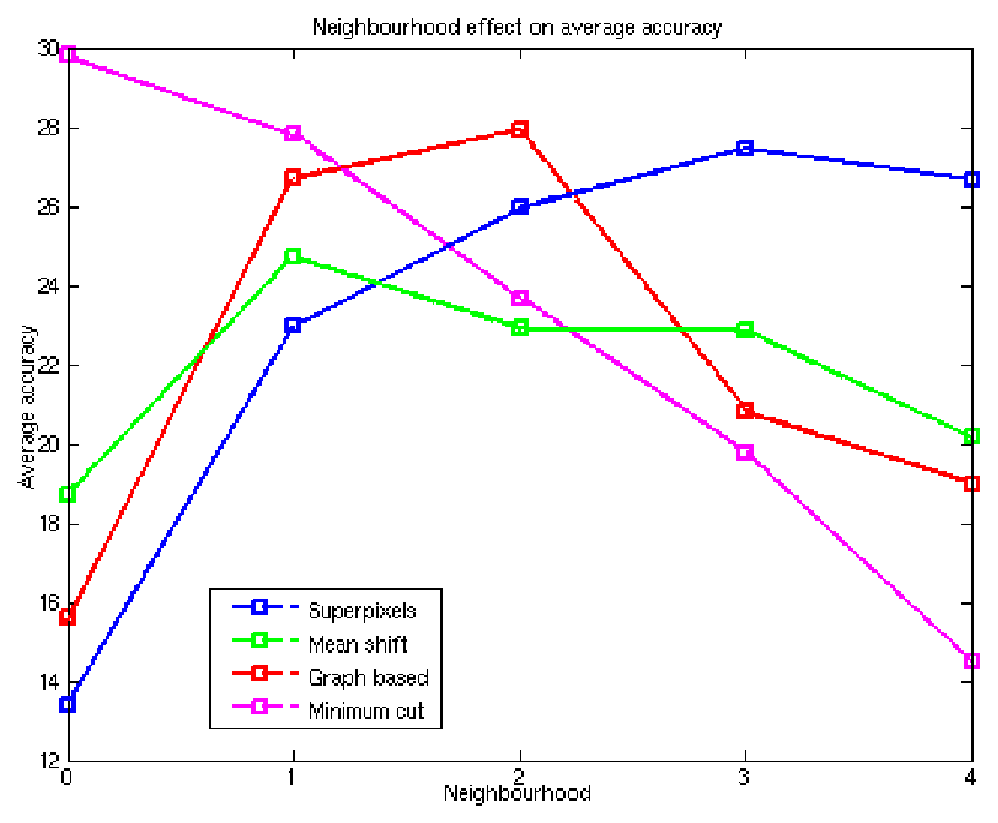
\includegraphics[scale=.33]{./Figures/neigh_acc.eps}
\centering
\caption{Effect of increasing neighborhood values on the average accuracies (Best viewed in colors).}
\label{fig:neigh_effect}
\end{figure}

Figure \ref{fig:neigh_effect} illustrates two important conclusions. First, large segments improve the
results. This conclusion is based on the observation of increasing the overall average accuracy in case of
(i) the large segments generated by the normalized cut technique, and
(ii) the generated segments using the superpixels or mean-shift methods when taking larger neighborhood
size into account.

The second conclusion is that up to a certain limit, increasing the size of the segments or the neighborhood,
decrease the final average accuracy. We attribute this to the loss of semantic information due to the combination
of segments that are no longer related to each others. Consequently, our target is to find a criteria to decide
whether combining smaller segments or splitting larger ones is more useful.

After we had these conclusions we aim to apply our proposed approach for combining multiple segmentations.
Assume we have $N$ segmentations $S_i$, where $i = 1, ..., N$ and each of the segmentations correspond to
$S_i = \bigcup_{j=1}^{C_i}T_{ij}$, where $T_{ij}$ is a segment in the segmentation $S_i$ and $C_i$ is the number
of segments obtained from the segmentation $S_i$. Our objective is to obtain a better segmentation
$S^* = \bigcup_{k=1}^{C^*}T_k^*$, where $T^*_k$ is a segment in our final set of optimized segments and
$C^*$ is the total number of optimized segments. Segmentation $S^*$ should satisfy the following criteria:

\begin{enumerate}
\item
The segments of the final segmentation should be as large as possible. In other words, we need to minimize $C^*$.
\item
The segments should be ``good'' segments. In our context, we defined a ``good segment'' as the largest set of
connected pixels that belong to the same object.
\end{enumerate}

Consequently, our motivation for combining segmentations is to start looking for the large segments and then check
if this segment is a ``good'' segment. We applied a greedy algorithm that favors large segments and check if they pass a
certain criteria of ``goodness''.
Our proposed approach is described as follows: Examine the largest segment obtained from all segmentations methods and
check whether this segment is a ``good'' segment. If the segment is ``good'', we include it in our final segmentation
(Add to $S^*$). Otherwise, we try to segment it recursively using the least number of segments from the other segmentations.
Similarly, we segment the remaining part of the image.

To this end, we need to determine whether the generated segments are ``good'' or not. To do this, we investigate several
``goodness'' evaluation criteria. First, we studied the possibility of assuming that the color of each region should follow
a normal distribution. However, this ``goodness'' criteria didn't hold on real images as shown in figure \ref{fig:histn}.
Second, we examined the unimodality test to check whether the distribution of the histogram of each RGB channel follow a
unimodal function. We use Dip test \cite{dip-unimodality} for unimodality. Although the resulting segments were slightly
better than those obtained using the normality test, it also fails to handle real images' segments as in figure \ref{fig:histn}.
In addition, we also investigated the outliers detection and the Ridge based Distribution Analysis (RAD) methods.
We'll describe these techniques in more details in the next sections.

\begin{figure}[!t]
\centering
\subfigure[] {
    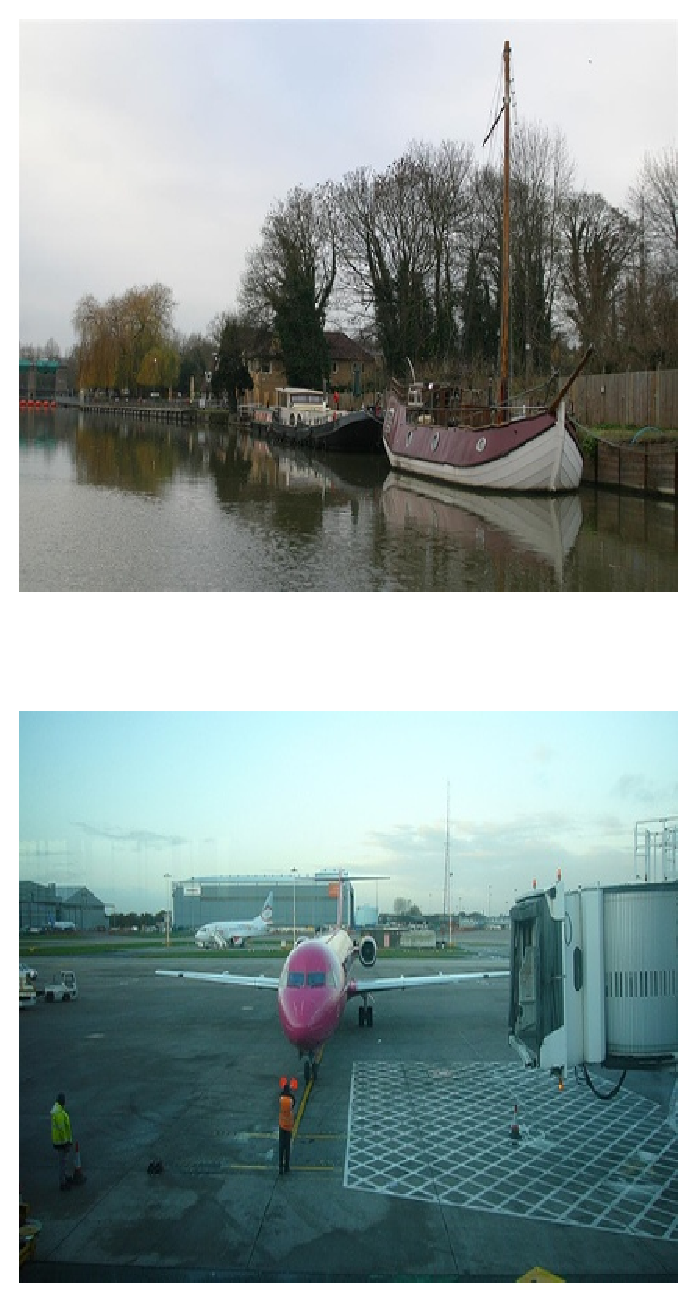
\includegraphics[width=70pt,height=85pt]{./Figures/orgnormality2.eps}
    \label{fig:orgn}
}
\subfigure[] {
    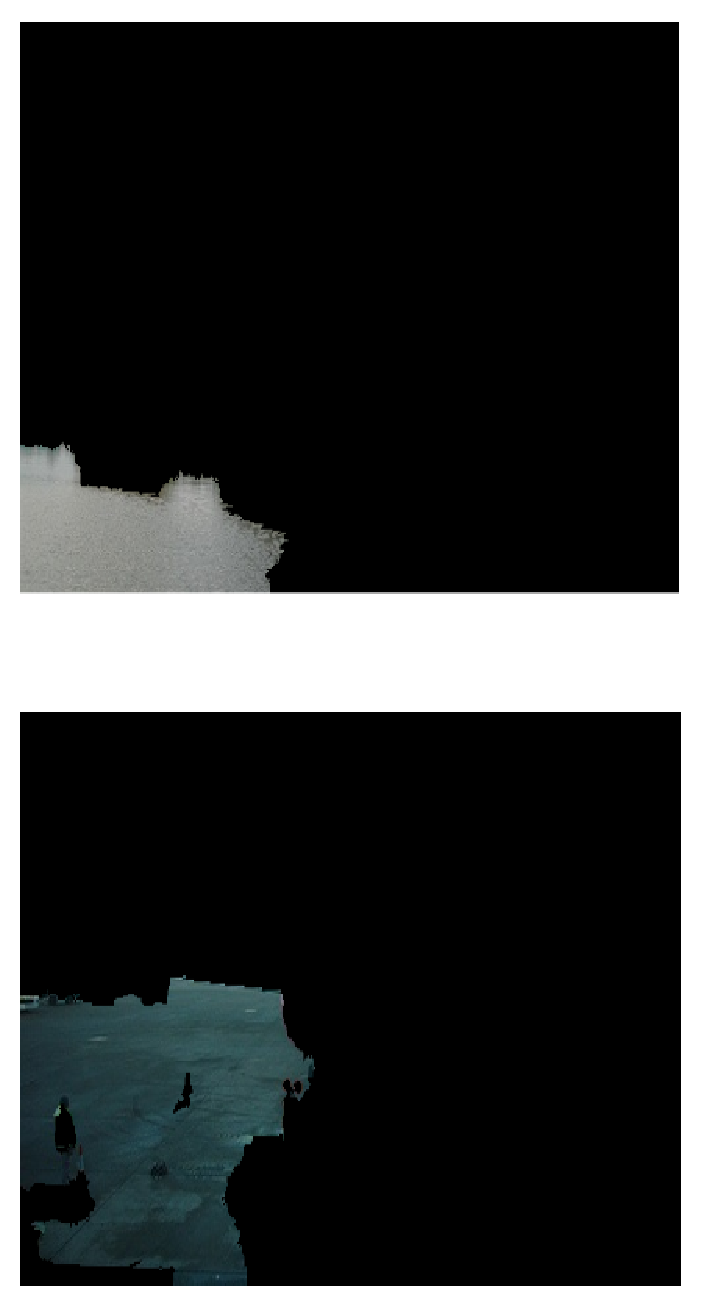
\includegraphics[width=70pt,height=85pt]{./Figures/segnormality2.eps}
    \label{fig:segn}
}
\subfigure[] {
    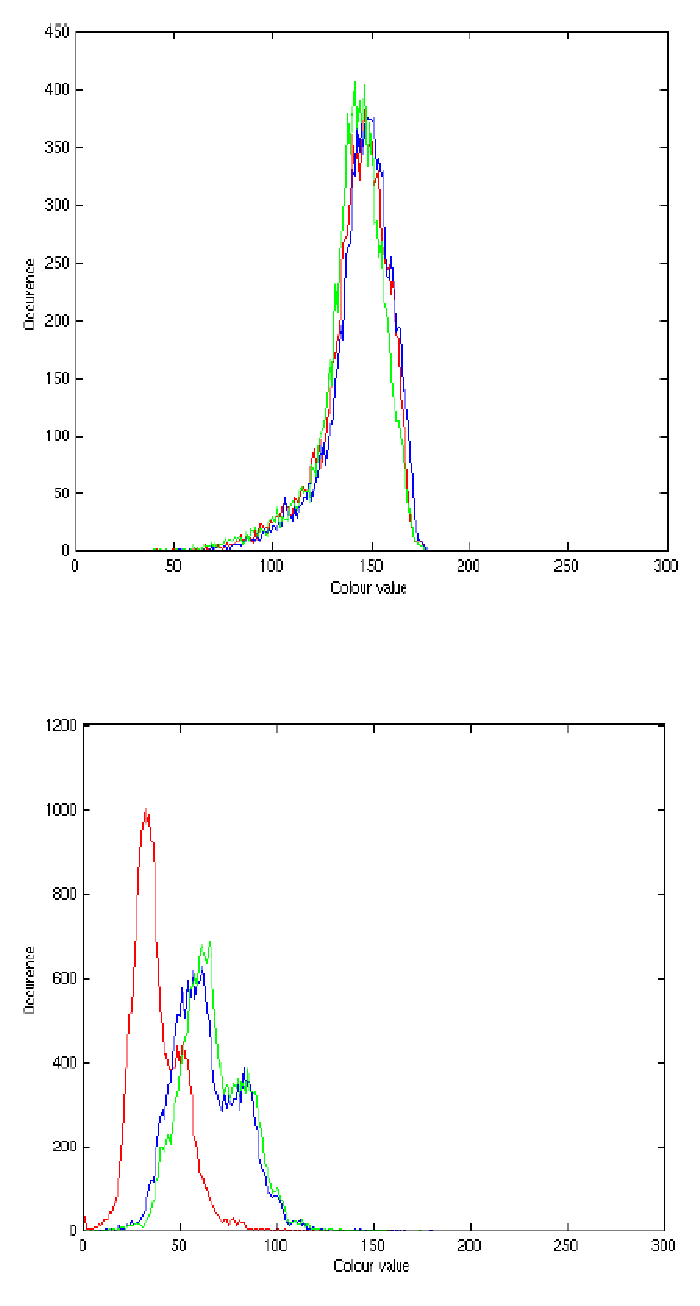
\includegraphics[width=70pt,height=85pt]{./Figures/histnormality2.eps}
    \label{fig:histn}
}
\caption{(a) Original images (b) Current largest segments (c) Histograms from every channel. As we can see the first image
can be approximated into a normal distribution or a unimodal distribution while the second one fails in that test.}
\label{fig:colorhists}
\end{figure}

\subsection{Good Segments Evaluation Using Outliers Finding}

As defined by \cite{grubbs-1969}, ``An outlying observation, or outlier, is one that appears to deviate markedly
from other members of the sample in which it occurs.'' In our work, we consider a segment to be ``good'' if the
fraction of outliers inside this segment is below a certain threshold.
We performed a series of experiments to empirically determine the best value for the tolerance of outliers
inside the segment. Results have shown that a segment is considered ``good'' if the number of outliers lying
inside is less than $2\%$ of the number of pixels in the segment.

Although outliers detection worked well in detecting the segments shown in Figure
\ref{fig:segn}, they didn't work on detecting the segments that contain variations
in shadows and highlights. Consequently, we examined other evaluation methods
that work well in the presence of shadows and illuminations. For this purpose, we use the
RAD evaluation method due to its robustness to shadows and highlights.

\subsection{Good Segments Evaluation Using RAD}

We use the RAD method \cite{1478239} for obtaining image
segmentations in the presence of shadows and highlights. This method is based on
the insight that the distributions formed by a single-colored object have a
physically determined shape (i.e. follow the same ridge) in the color histogram space \cite{Sha85}.
To capture these ridges Vazquez et al. \cite{1478239} proposed a new Ridge based
Distribution Analysis (RAD) to find the set of ridges representative of the dominant colors in the image.

We model the region ``segment'' by its set of dominant colors (DC). This DC is described
by a distribution in histogram-space. We assume that if this segment contains only 1 DC
then this segment is a ``good'' segment as this segment contains only 1 semantic object.
Based on this technique, the evaluation method becomes very robust to shadows and highlights
and becomes closely related to the physical features of each segment than the previously
investigated methods.

\section{Experimental results}

In figure \ref{fig:mix_allsegs} we show some qualitative results to the images resulting from the
various segmentation techniques as well as the two ways discussed for combining segments and
evaluating segments quality.

\begin{figure}[!t]
\centering
\subfigure[] {
    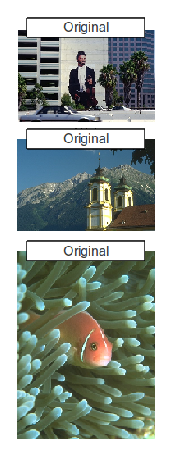
\includegraphics[width=48pt,height=170pt]{./Figures/orgseg.eps}
    \label{fig:org}
}
\subfigure[] {
    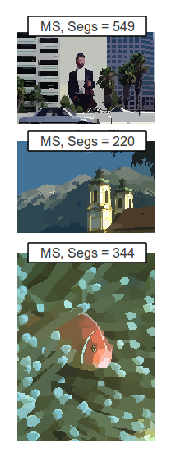
\includegraphics[width=48pt,height=170pt]{./Figures/msseg.eps}
    \label{fig:ms}
}
\subfigure[] {
    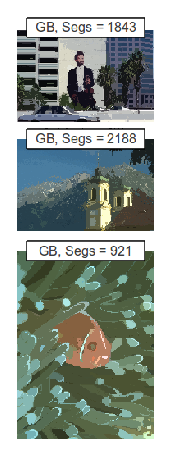
\includegraphics[width=48pt,height=170pt]{./Figures/gbseg.eps}
    \label{fig:gb}
}
\subfigure[] {
    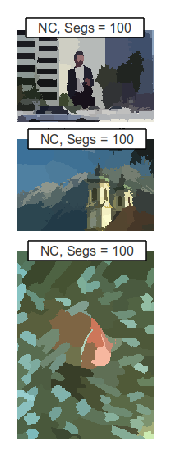
\includegraphics[width=48pt,height=170pt]{./Figures/ncseg.eps}
    \label{fig:nc}
}
\subfigure[] {
    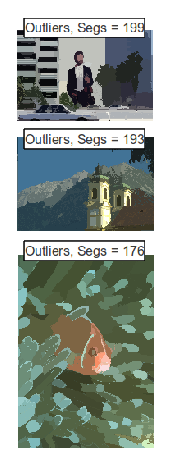
\includegraphics[width=48pt,height=170pt]{./Figures/outliersseg.eps}
    \label{fig:mix_out}
}
\subfigure[] {
    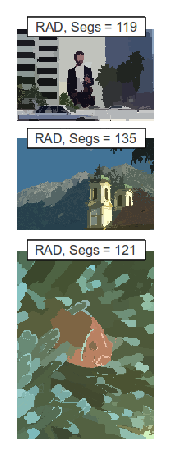
\includegraphics[width=48pt,height=170pt]{./Figures/radseg.eps}
    \label{fig:mix_rad}
}
\caption{(a) Original image.
(b) Mean-shift segmentation.
(c) Graph-Based segmentation.
(d) Normalized-Cut segmentation.
(e) Evaluation with Outliers.
(f) Evaluation with RAD.}
\label{fig:mix_allsegs}
\end{figure}

We also perform a series of experiments on the standard Berkeley Segmentation Dataset and
Benchmark \cite{MartinFTM01}. We evaluate the performance of the three considered segmentation methods with
our newly proposed segmentation methods. Our method combines the complementary information obtained by all the
considered segmentation methods using the Outliers and RAD criteria for segments ``goodness'' evaluation. Our combination
method's main motivation is getting the largest possible segments as a motivation to improve the task of \textit{object
class segmentation}.

We evaluate four different error measurements for evaluating the quality of the segments
generated by our approach. These four error measures are: First, the Probabilistic Rand Index
(PRI) \cite{Unnikrishnan_2007_5789}, which counts the fraction of pairs of pixels whose labellings are
consistent between the computed segmentation and the ground truth, averaging across
multiple ground truth segmentations to account for scale variation in human perception.
The second error measure is the Variation of Information (VoI) \cite{citeulike:3906686}.
It defines the distance between two segmentations as the average conditional entropy
of one segmentation given the other, and thus roughly measures the amount of randomness
in one segmentation which cannot be explained by the other. The third is the Global
Consistency Error (GCE) \cite{MartinFTM01} that measures the extent to which one
segmentation can be viewed as a refinement of the other. Segmentations which are related
in this manner are considered to be consistent, since they could represent the same
natural image segmented at different scales. The fourth measure is the Boundary
Displacement Error (BDE) by \cite{649319}. It measures the average displacement error of
boundary pixels between two segmented images. Particularly, it defines the error of one
boundary pixel as the distance between the pixel and the closest pixel in the other
boundary image.

Table \ref{tab:seg_bench} demonstrates that our proposed segmentation method improves both of the
PRI and the VoI error measures. Whether evaluating our segments quality with outliers or RAD evaluation criteria.
We attribute this to the fact that  PRI and VoI are clearly concerned about comparing segments entirely with the ground truth segments.
This justifies our motivation behind our proposed segmentation method which is based on improving the size and the quality of the segment.
In contrary, GCE and BDE measures don't perform well on our approach.
These measures are mainly concerned about the boundaries of the segments which our approach doesn't take into concern.

\begin{table}[!t]
\centering
\begin{tabular}
{|c||c|c|c|c|}
\hline
                              & PRI             & VoI             & GCE             & BDE              \\\hline
Mean-Shift                    & 0.7424          & 4.5293          & \textbf{0.0842} & \textbf{14.2716} \\\hline
Graph-Based                   & 0.7082          & 5.1148          & 0.1150          & 17.2428          \\\hline
Normalized-cut                & 0.7079          & 4.1370          & 0.1153          & 14.7337          \\\hline
Combine + Outliers Evaluation & 0.7462          & 3.7264          & 0.1380          & 14.7730          \\\hline
Combine + RAD Evaluation      & \textbf{0.7483} & \textbf{3.5364} & 0.1433          & 14.8047          \\\hline
\end{tabular}
\caption{Segmentation benchmarks results for the Berkeley Segmentation Dataset and
Benchmark. 4 error measures were considered for 4 different segmentations.}\label{tab:seg_bench}
\end{table}

\section{Conclusions}

We have demonstrated the effect of using multiple segmentations on improving the segments and hence
improving the applications that use image segmentations as a prerequisite. Our approach aims to select
the ``good'' segments from amongst a set of segmentations. We've investigated two criteria for measuring segments' goodness.
We believe we can still improve our resulting segmentations by investigating more criteria for measuring goodness.
For instance, for the JSEG segmentation \cite{jseg:462311}, the criterion chosen for good segmentations evaluation is the spatial relation existing
between the pixels in the image space. Another way is to use the color boosting algorithm introduced in
\cite{Weijer05boostingcolor} and consider a segment ``good'' if the number of salient points is below a certain threshold.

\bibliographystyle{splncs03}
\bibliography{egbib}

\end{document}
